
% ----------------------------------------------------------------------
%  Set the document class
% ----------------------------------------------------------------------
\documentclass[11pt,a4paper,twoside]{article}

% ----------------------------------------------------------------------
% Define external packages, language, margins, fonts and new commands
% ----------------------------------------------------------------------
%\input{preamble} 
\usepackage[utf8]{inputenc}   % <<<<< Linux
\usepackage[english]{babel} % <<<<< English
\usepackage{notoccite}
\usepackage{amsmath}
\usepackage{amssymb}
\usepackage[labelfont=bf]{caption}
\usepackage[skip=0.5\baselineskip]{caption}
\usepackage{float}
\hyphenation{GTKWave}
\usepackage{listings}
\usepackage[all]{nowidow}

%blind text
\usepackage{lipsum}

\usepackage{graphicx}
\graphicspath{{./}{../../figlib/}{../mat/}{../sim/}}
\def\FontLn{% 16 pt normal
  \usefont{T1}{phv}{m}{n}\fontsize{16pt}{16pt}\selectfont}
\def\FontLb{% 16 pt bold
  \usefont{T1}{phv}{b}{n}\fontsize{16pt}{16pt}\selectfont}
\def\FontMn{% 14 pt normal
  \usefont{T1}{phv}{m}{n}\fontsize{14pt}{14pt}\selectfont}
\def\FontMb{% 14 pt bold
  \usefont{T1}{phv}{b}{n}\fontsize{14pt}{14pt}\selectfont}
\def\FontSn{% 12 pt normal
  \usefont{T1}{phv}{m}{n}\fontsize{12pt}{12pt}\selectfont}

% Use Arial font as default
%
\renewcommand{\rmdefault}{phv}
\renewcommand{\sfdefault}{phv}
\usepackage{geometry}	
\geometry{verbose,tmargin=2.5cm,bmargin=2.5cm,lmargin=2.5cm,rmargin=2.5cm}

%\usepackage{setspace}
%\renewcommand{\baselinestretch}{1.5}

\usepackage[pdftex]{hyperref} % enhance documents that are to be
                              % output as HTML and PDF
\hypersetup{colorlinks,       % color text of links and anchors,
                              % eliminates borders around links
%            linkcolor=red,    % color for normal internal links
            linkcolor=black,  % color for normal internal links
            anchorcolor=black,% color for anchor text
%            citecolor=green,  % color for bibliographical citations
            citecolor=black,  % color for bibliographical citations
%            filecolor=magenta,% color for URLs which open local files
            filecolor=black,  % color for URLs which open local files
%            menucolor=red,    % color for Acrobat menu items
            menucolor=black,  % color for Acrobat menu items
%            pagecolor=red,    % color for links to other pages
            pagecolor=black,  % color for links to other pages
%            urlcolor=cyan,    % color for linked URLs
            urlcolor=black,   % color for linked URLs
	          bookmarks=true,         % create PDF bookmarks
	          bookmarksopen=false,    % don't expand bookmarks
	          bookmarksnumbered=true, % number bookmarks
	          pdftitle={report},
            pdfauthor={Andre C. Marta},
%            pdfsubject={Thesis Title},
%            pdfkeywords={Thesis Keywords},
            pdfstartview=FitV,
            pdfdisplaydoctitle=true}

\usepackage[numbers,sort&compress]{natbib} % <<<<< References in numbered list [1],[2],...
\usepackage{subcaption} 
\usepackage{mdframed}

%%%%%%%%%%%%%%%%%%%%%%%%%%%%%%%%%%%%%%%%%%%%%%%%%%%%%%%%%%%%%%%%%%%%%%%%
%     Begin Document                                                   %
%%%%%%%%%%%%%%%%%%%%%%%%%%%%%%%%%%%%%%%%%%%%%%%%%%%%%%%%%%%%%%%%%%%%%%%%


\begin{document}

% Set plain page style (no headers, footer with centered page number)
\pagestyle{plain}

% Set roman numbering (i,ii,...) before the start of chapters
%\pagenumbering{roman}

% ----------------------------------------------------------------------
%  Cover page
% ----------------------------------------------------------------------
%%%%%%%%%%%%%%%%%%%%%%%%%%%%%%%%%%%%%%%%%%%%%%%%%%%%%%%%%%%%%%%%%%%%%%%%
%                                                                      %
%     File: Thesis_FrontCover.tex                                      %
%     Tex Master: Thesis.tex                                           %
%                                                                      %
%     Author: Andre C. Marta                                           %
%     Last modified :  2 Jul 2015                                      %
%                                                                      %
%%%%%%%%%%%%%%%%%%%%%%%%%%%%%%%%%%%%%%%%%%%%%%%%%%%%%%%%%%%%%%%%%%%%%%%%
\thispagestyle {empty}

% IST Logo - Signature A
% parameters: bb=llx lly urx ury (bounding box), width=h_length, height=v_length, angle=angle, scale=factor, clip=true/false, draft=true/false. 
\includegraphics[bb=9.5cm 11cm 0cm 0cm,scale=0.29]{IST_A_CMYK_POS}

\begin{center}
%
% Figure (Image or plot)
\vspace{1.0cm}
% height = 50 mm
%\includegraphics[height=50mm]{Figures/Airbus_A350.jpg}

% Title, author and degree
\vspace{1cm}
{\FontLb Instituto Superior Técnico, University of Lisbon} \\ % <<<<< UNIVERSITY
\vspace{1cm}
{\FontLb Integrated Master in Aerospace Engineering} \\ % <<<<< MASTER'S DEGREE
\vspace{1cm}
{\FontSn Circuit Theory and Electronics Fundamentals} \\ % <<<<< COURSE
\vspace{1cm}
{\FontSn Joana Matos (95799), Ricardo Abreu (95842), Vasco Emídio (95856)} \\ % NAMES
\vspace{1cm}
{\FontSn First Laboratory Report} \\
\vspace{1cm}
{\FontSn March 24, 2021} \\ % <<<<< EDIT DATE (corresponds to date of oral examination)
%
\end{center}



% ----------------------------------------------------------------------
% Dedication page (optional)
% ----------------------------------------------------------------------
%\input{dedication} 
%\cleardoublepage

% ----------------------------------------------------------------------
%  Acknowledgments (optional)
% ----------------------------------------------------------------------
%\input{acknowledgements}
%\cleardoublepage

% ----------------------------------------------------------------------
%  Abstract (both in English and Portuguese)
% ----------------------------------------------------------------------
%\input{resumo} 
%\cleardoublepage

%\input{abstract} 

% ----------------------------------------------------------------------
%  Table of contents, list of tables, list of figures and nomenclature
% ----------------------------------------------------------------------

% Table of contents
%
\tableofcontents

% List of tables
%\addcontentsline{toc}{section}{\listtablename}
%\listoftables
%\cleardoublepage 

% List of figures
%\addcontentsline{toc}{section}{\listfigurename}
%\listoffigures
%\cleardoublepage 

% Set arabic numbering (1,2,...) after preface
%
%\setcounter{page}{1}
%\pagenumbering{arabic}

% ----------------------------------------------------------------------
%  Body
% ----------------------------------------------------------------------

\section{Introduction}
\label{sec:introduction}
% state the learning objective 
The objective of this laboratory assignment is to study a circuit containing a
DC voltage source $V_a$, seven resistors, a voltage-controlled current source $I_b$ and
a current-controlled voltage source $V_c$. The components of this circuit are distribuited 
by 4 elementary meshes and 8 nodes, as seen in Figure~\ref{fig:circuit}. 

In order to analyse the circuit, the following data were obtained by running the supplied Python script: 

\textit{Units for the values:} V, mA, kOhm and mS\par
\textit{Values:} 

R1 = 1.00147062639\par
R2 = 2.0078068512\par
R3 = 3.11269704405\par
R4 = 4.10609573471\par
R5 = 3.02670672634\par
R6 = 2.01292455078\par
R7 = 1.02905244808\par
Va = 5.24842063411\par
Id = 1.04086013403\par
Kb = 7.21413591579\par
Kc = 8.01455113996


In Section~\ref{sec:analysis}, a theoretical analysis of the circuit, performed on Octave
using the mesh and node methods, is presented. In Section~\ref{sec:simulation}, the 
circuit is analysed by simulation, using NGSpice, and the results are compared to 
the theoretical results obtained in Section~\ref{sec:analysis}. The conclusions 
of this study are outlined in Section~\ref{sec:conclusion}.

\begin{figure}[H] \centering
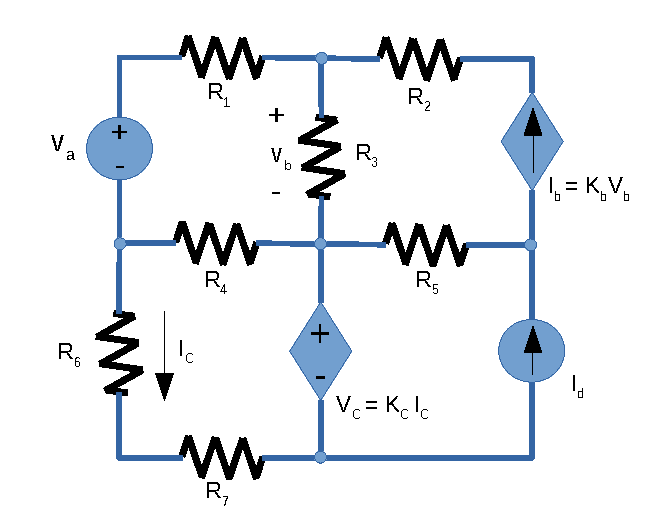
\includegraphics[width=0.4\linewidth]{circuit.pdf}
\caption{Circuit which will be analysed during this laboratory assignment.}
\label{fig:circuit}
\end{figure}



\section{Theoretical Analysis}
\label{sec:analysis}
In this section, the circuit shown in Figure~\ref{fig:circuit} is analysed theoretically.
It is important to notice that the purpose is to build a band pass filter circuit using an OPAMP.
This way, the considered circuit has a high pass filter, a signal amplifier (OPAMP) and a low pass filter in series,
where the capacitor C1 and the resistor R1 act as a high pass filter, while capacitor C2 and resistor R2 function as a low pass filter.

Thus, We will begin by computing the gain, input and output impedances at the central frequency.
Then, we will compute the frequency response Vo(f)/Vi(f) , using the incremental circuit, 
solving the circuit for a frequency vector in log scale with 10 points per decade, from 10Hz to 100MHz.
%It is important to notice that, in this analysis, the OP-AMP used is considered ideal, wich means that

%--------------------------------------------------------------------------------------------
\subsection{Gain, Input and Output Impedances at central frequency}
In this subsection, we will compute the gain, input and output impedances at the central frequency.

First, we will calculate low and high cutoff frequencies, $w_L$ and $ w_H$, respectively, as well as central frequency, $w_O$, which are given by:
\begin{equation}
	w_L=\frac{1}{R_{1} \cdot C_{1}}
\end{equation}
\begin{equation}
	w_H=\frac{1}{R_{2} \cdot C_{2}}
\end{equation}
\begin{equation}
	w_O=\frac{1}{ \sqrt{w_{L} \cdot w_{H}}}
\end{equation}

Their values are presented in the table below:
\begin{table}[H]
  \centering
  \begin{tabular}{|l|r|}
     \hline    
    {\bf Name} & {\bf Value} \\ \hline   
    $w_{L}$ & 5.000000e+03 rad/s \\ \hline
$w_{H}$ & 9.090909e+03 rad/s \\ \hline
$w_{O}$ & 6.741999e+03 rad/s \\ \hline
$f_{O}$ & 1.073022e+03 Hz \\ \hline

  \end{tabular}
  \caption{Frequencies}
  \label{tab:freq}
\end{table}

Now we can determine the gain at central frequency, wich is given by the following equation:
\begin{equation}
	T_{w_O}=\frac{R_1\cdot C_1 \cdot jw_O}{1+R_1*C_1*jw_O}\cdot(1+ \frac{R_3}{R_4}) \cdot \frac{1}{1+R_2 \cdot C_2\cdot jw_O}
\end{equation}
, where $R_4$ is the $R_{4a}$ and $R_{4b}$ equivalent resistor.

As well as $Z_{in}$ and $Z_{out}$, at the central frequency, are determined by:
\begin{equation}
	Z_{in}=\frac{R_1\cdot C_1 \cdot jw_O}{1+R_1*C_1*jw_O}\cdot(1+ \frac{R_3}{R_4}) \cdot \frac{1}{1+R_2 \cdot C_2\cdot jw_O}
\end{equation}
\begin{equation}
	Z_{out}=R_1+\frac{1}{jw_O*C_1}
\end{equation}

The results are shown in tables~\ref{tab:results1} and~\ref{tab:results2}:
\begin{table}[H]
  \centering
  \begin{tabular}{|l|r|}
     \hline    
    {\bf Name} & {\bf Value} \\ \hline   
    $Z_{in}$ & 9.090909e+02 + j-6.741999e+02 Ohm \\ \hline
$Z_{out}$ & 6.451613e+02 + j-4.784644e+02Ohm \\ \hline
$|Z_{in}|$ & 1.131809e+03 Ohm \\ \hline
$|Z_{out}|$ & 8.032193e+02 Ohm \\ \hline

  \end{tabular}
  \caption{Impedances at central frequency}
  \label{tab:results1}
\end{table}
\begin{table}[H]
  \centering
  \begin{tabular}{|l|r|}
     \hline    
    {\bf Name} & {\bf Value} \\ \hline   
    $AV_{HP}$ & -1.903317e+00 dB \\ \hline
$AV_{OPAMP}$ & 4.440216e+01 dB \\ \hline
$AV_{LP}$ & -1.903317e+00 dB \\ \hline
$AV$ & 4.059553e+01 dB \\ \hline

  \end{tabular}
  \caption{Gain at central frequency}
  \label{tab:results2}
\end{table}

\subsection{Frequency response Vo(f)/Vi(f)}
Now, considering the transfer function $T(s)$, it is given by:
\begin{equation}
	T(s)=\frac{V_out(s)}{V_in(s)}=1+\frac{Z_{in}(s)}{Z_{out}(s)}=\frac{R_1\cdot C_1 \cdot s}{1+R_1*C_1*s}\cdot(1+ \frac{R_3}{R_4}) \cdot \frac{1}{1+R_2 \cdot C_2\cdot s}
\end{equation}
, where $\frac{R_1\cdot C_1 \cdot s}{1+R_1*C_1*s}$, $1+\frac{R_3}{R_4}$ and $\frac{1}{1+R_2\cdot C_2\cdot s}$ represent
the gain at high pass filter, OP-AMP and low pass filter, respectively.

This way, the gain frequency response is plotted in the figure below.
\begin{figure}[H] \centering
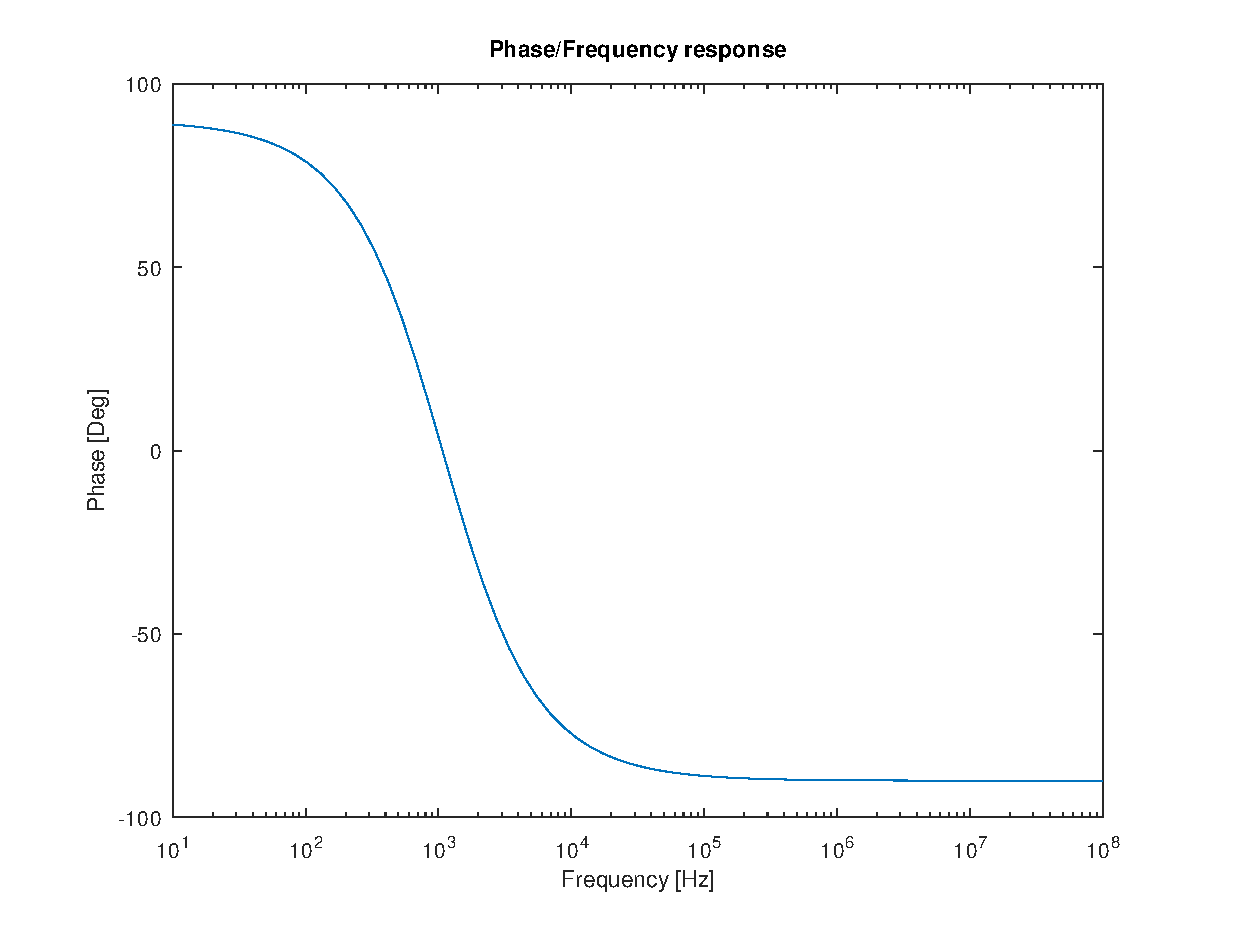
\includegraphics[width=0.6\linewidth]{phase_response.eps}
\caption{Phase Frequency Response}                         %%%%%%%%%%LEGENDA
\label{fig:phasef}
\end{figure}
\begin{figure}[H] \centering
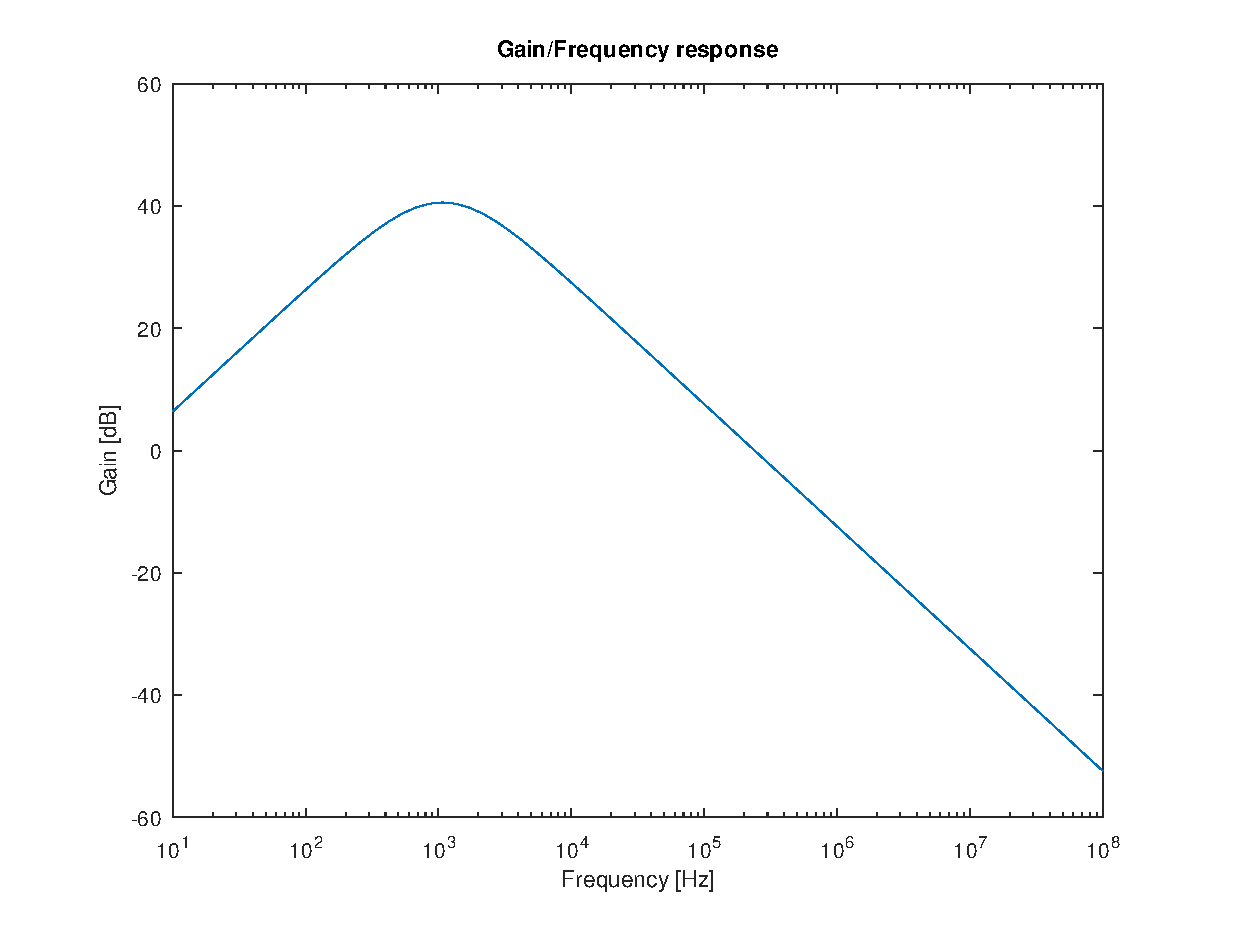
\includegraphics[width=0.6\linewidth]{gain_response.eps}
\caption{Gain Frequency Response}                         %%%%%%%%%%LEGENDA
\label{fig:gainf}
\end{figure}
As we can see there is a maximum for the frequencies in the central frequency, wich is near to 1KHz, otherwise low and high frequencies have a low gain. That was expected because
both low and high frequencies were blocked by high and low pass filters.

%\subsection{Comparison}

%Table~\ref{tab10:sim} presents the simulation results for the circuit under analysis.

%\begin{table}[H]
%  \centering
%  \begin{tabular}{|l|r|}
%    \hline    
%    {\bf Name} & {\bf V or dB} \\ \hline
%    \input{../sim/sim_tab}
%  \end{tabular}
%  \begin{tabular}{|l|c|}
%    \hline
%    {\bf Impedance} & {\bf kOhms} \\ \hline
%    zin & 2.236262e+00\\ \hline

%  \end{tabular}
%  \begin{tabular}{|l|c|}
%    \hline
%    {\bf Impedance} & {\bf kOhms} \\ \hline
%    \input{../sim/output_tab2}
%  \end{tabular}
%    \caption{Simulation Results.}
%    \label{tab10:sim}
%\end{table}

%Comparing with the theoretical ones, we can see that they are slightly different, result of the fact that the theoretical model is an approximation and the transistors used in NGSpice were real. However, the results obtained are satisfatory!


\section{Simulation Analysis and Comparison with Theoretical Results}
\label{sec:simulation}

\subsection{Transient Analysis}


Figure~\ref{fig:trans2} shows the simulated transient analysis results for input voltage of the secondary circuit,
the envelope detector output voltage, $V_3$, the voltage regulator output voltage, $V_4$ 
and the average voltage difference, $V_4$-12 Volts.

\begin{figure}[H] \centering
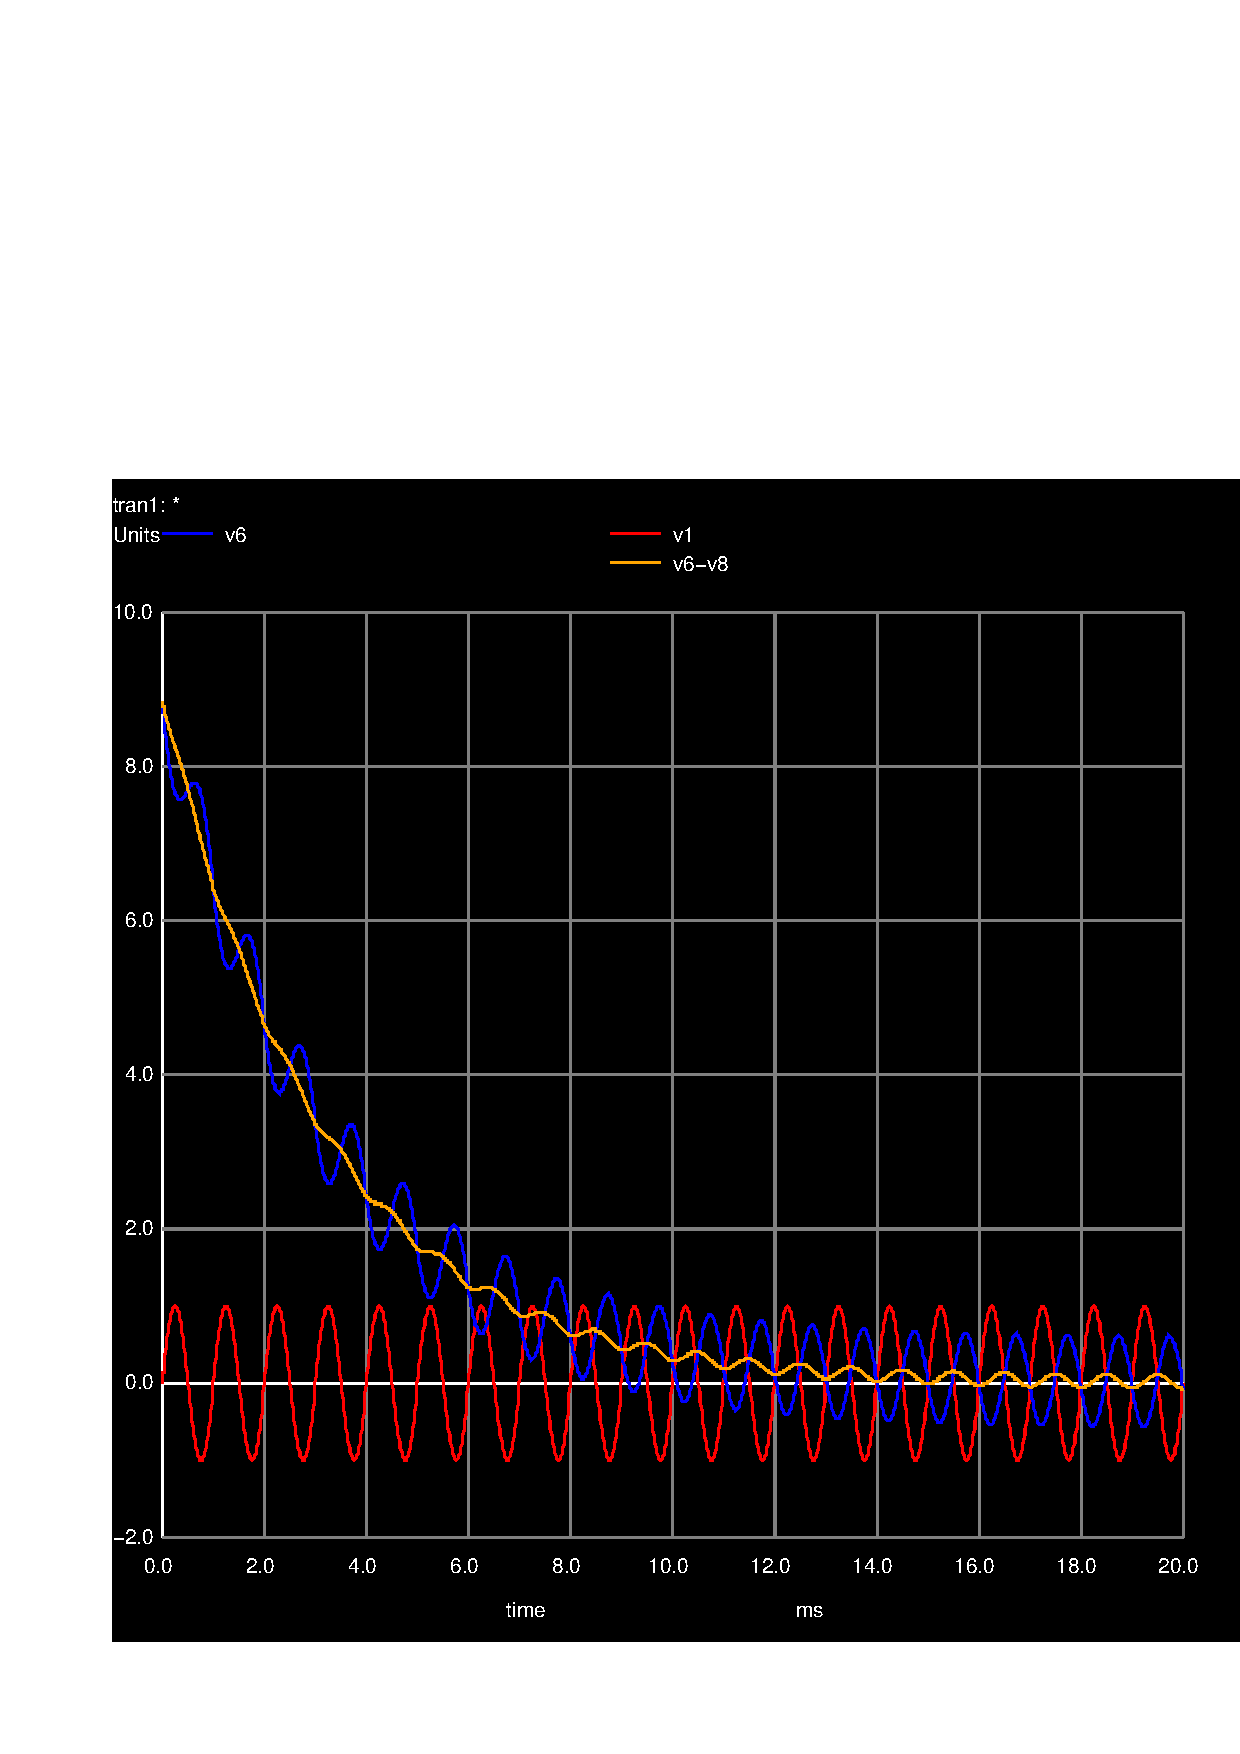
\includegraphics[width=0.4\linewidth]{trans2.pdf}
\caption{Transient input voltage of the secondary circuit and transient output voltage of both the envelope detector and 
voltage regulator and the average voltage difference.}
\label{fig:trans2}
\end{figure}

By analysing the result of the simulation we notice that the output solution resulted in an aproximated sinusoidal 
fuction: in fact, because of the average voltage is not ideal, the curve has an upward sinusoidal motion and 
a downward motion described by a negative exponential. The input voltage is described by a sinusoidal fuction, as expected. 
As far as the result is concerned, the form of the theoretical solution match the one obtained by NGSpice. 
Note that, because of the scale, we can not see the wave form of the ripple voltage and voltage difference because 
they are very small, which means that we obtained a decent result for 2 of the 3 parameters that influence the merit.


	Table~\ref{tab1:op} shows the measured results for the maximum, minimum and average output voltage of the circuit $V_4$. 
	Notice that the values on the right were obtained by Octave, therefore they are the theoretical values, which we already 
	mentioned previously but, to facilitate the comparison between the simulation and theoretical values, we mentioned them again.

\begin{table}[H]
  \centering
  \begin{tabular}{|l|r|}
    \hline    
    {\bf Name} & {\bf Voltage[V]} \\ \hline
    \input{../sim/op1_tab}
  \end{tabular}
  \begin{tabular}{|l|r|}
    \hline    
    {\bf Node} & {\bf Voltage[V]} \\ \hline
    \input{../mat/V_tab}
  \end{tabular}
  \caption {Measured maximum $V_max$, minimum $V_min$ and average $V_avg$ output voltage of the circuit. 
  The values on the right are the theoretical values for the same voltages in the circuit.}
  \label{tab1:op}
\end{table}


	Compared to the theoretical analysis results, we notice that both simulation results are accurate, except for the last 
decimal places, as a consequence of the cientific notation and the number of significative algharisms used by each program to 
present the results. Despite that, we realise that the values with more significant algharisms match correctly the rounded values.


	Table~\ref{tab2:op} shows the ripple voltage of the circuit and the average voltage difference
	between the output voltage and 12 Volts. Again, we show the theoretical values obtained for this step, 
	to make it easier to compare between simulation and theoretical values.


\begin{table}[H]
  \centering
  \begin{tabular}{|l|r|}
    \hline    
    {\bf Name} & {\bf Voltage[V]} \\ \hline
    \input{../sim/op2_tab}
  \end{tabular}
  \begin{tabular}{|l|r|}
    \hline    
    {\bf Name} & {\bf Voltage[V]} \\ \hline
    \input{../mat/Ripple_tab}
  \end{tabular}
  \caption{Ripple voltage $V_max$-$V_min$ and the average voltage difference $V_4$-12. The values on the right are the theoretical 
  values for the same voltages in the circuit.}
  \label{tab2:op}
\end{table}


Table~\ref{tab3:op} shows the total cost of the circuit and the figure of merit of the circuit. 
Note that we used the simulated voltage results to calculate the value of merit.


\begin{table}[H]
  \centering
  \begin{tabular}{|l|r|}
    \hline    
    {\bf Formula} & {\bf Merit} \\ \hline
    \input{../sim/op3_tab}
  \end{tabular}
  \caption{Figure of merit with a cost of 222.4 monetary units (MU).}
  \label{tab2:op}
\end{table}

By analising the figure of merit, we note that its value, considering the multiple results obtained for different values of the components and layots of the circuit, is
reasonable. Nevertheless, we consider the result not satisfying, since we obtained a merit of around 900 when we eliminated resistor $R_1$ and added 15 more diodes to the series
(reducing considerably the cost, the ripple and the average voltage difference). However, the AC/DC converter obtained would not be an efficient one, since it would have an enourmous
stabilization time and no resistor connected in parallel with the capacitor.



\section{Conclusion}
\label{sec:conclusion}

In this laboratory assignment the objective of analysing a RC circuit by determining its natural and forced solution has been achieved. The theoretical analysis was performed with the help of the Octave math tool and the circuit simulation using the Ngspice tool. In both analysis, we had to determine the operating point results for t$<$0 and t=0, and then apply the results obtained previously to plot the solutions, which were the time fuction of $v_6$, $v_s$ and the voltage in the capacitor $C$ and the respective frequency fuctions of their magnitudes and phases. The simulation results matched the theoretical results accurately - furthermore, because we use the time interval [-5;20]ms for the theoretical analysis, we can notice the discontinuities of some voltage values, which were previously explained in this report.

%\cleardoublepage

% ----------------------------------------------------------------------
%  Bibliography
% ----------------------------------------------------------------------
%\addcontentsline{toc}{section}{\bibname}
%\bibliographystyle{abbrvunsrtnat} % <<<<< SELECT IF USING REFERENCES BY NUMBER (CITATION ORDER)
%\bibliography{../../../BIBfile.bib}

% ----------------------------------------------------------------------
\end{document}
% ----------------------------------------------------------------------
